% \header{Our Approach}

% While diffusion models have shown promise for trajectory generation, existing approaches either lack task generalization or narrowly encode robot dynamics for specific tasks. Most importantly, they focus primarily on geometric constraints and collision avoidance, neglecting the crucial role of dynamics in physical execution.

\section{Proposed Work}

\begin{figure}
  \centering
    % \includegraphics[width=\columnwidth,height=0.75\columnwidth]{example-image-a}
    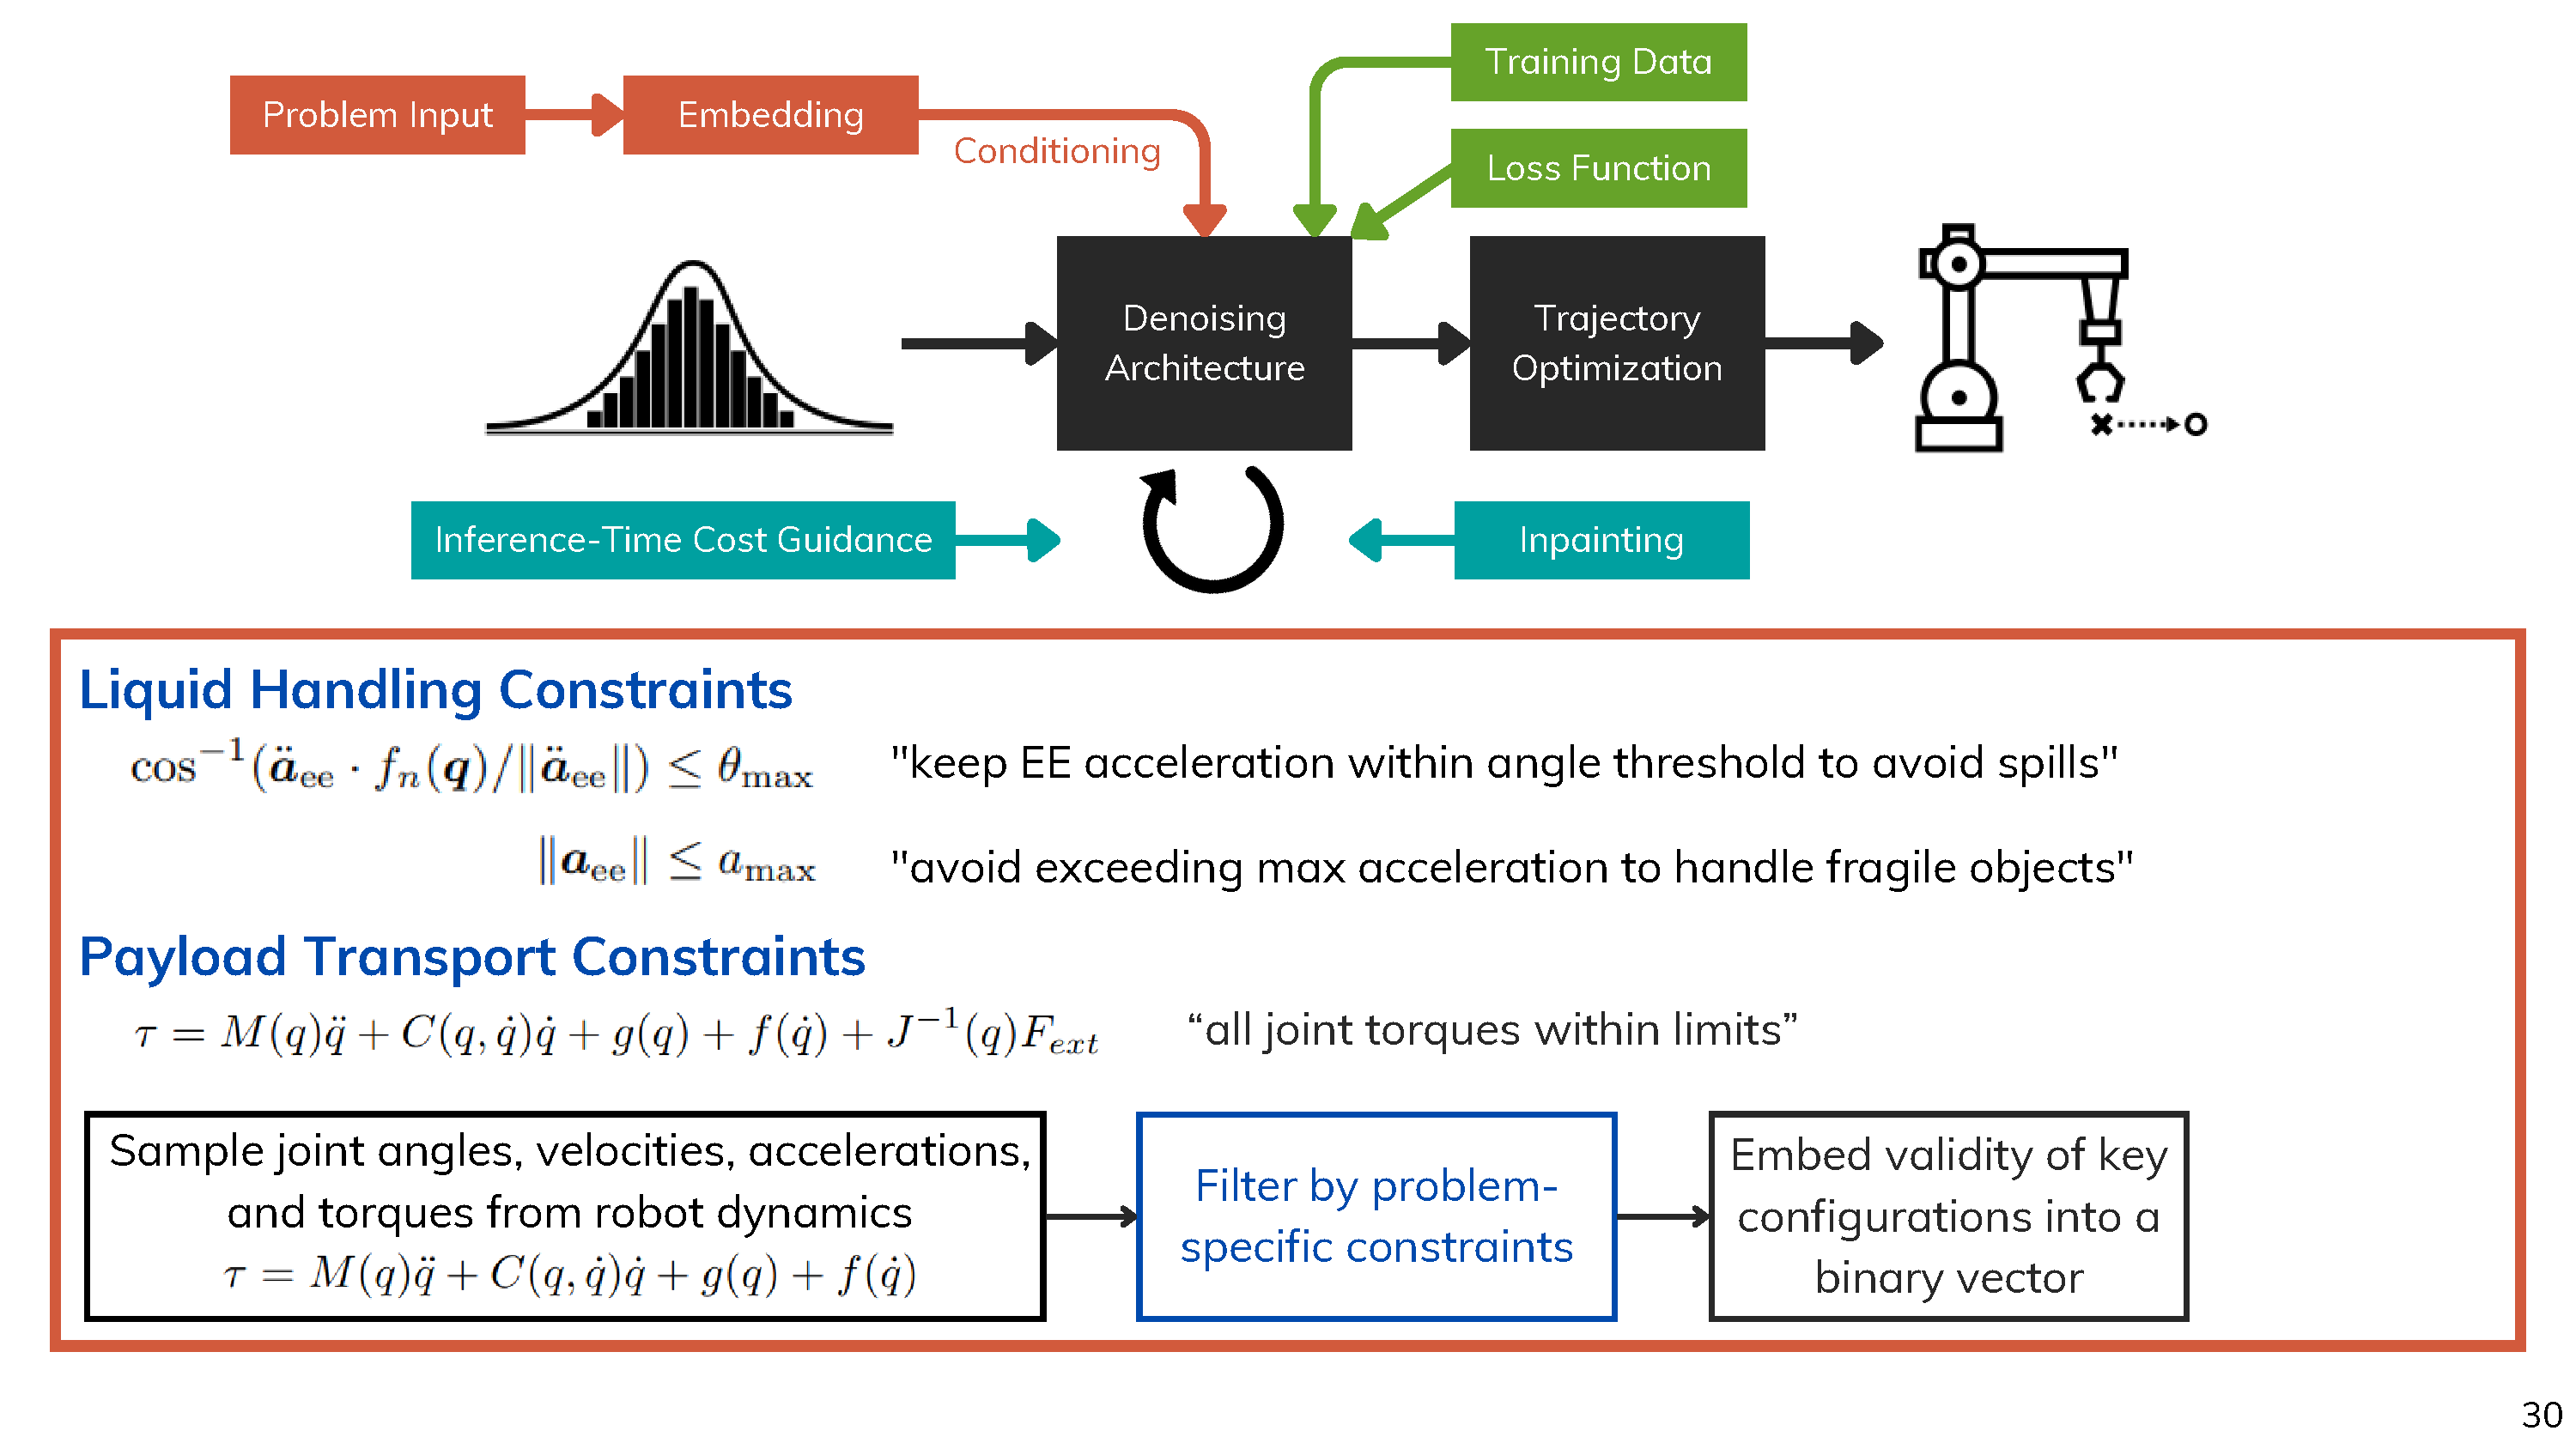
\includegraphics[width=\columnwidth]{graphics/new-diag.pdf}
  \caption{My proposed project involves generating near-admissible seed trajectories for optimization with kinematic and dynamic constraints. The sample conditioning mechanism makes the diffusion model applicable to a variety of trajectory optimization problems.}\label{fig:proposed}
\end{figure}

While prior work has demonstrated promising results in trajectory generation using diffusion models, existing approaches remain focused on geometric constraints \cite{sundaralingam2023curobo,seo2024presto}, are limited in task generalization \cite{ichnowski2020deep}, or implicitly encode robot dynamics for specific tasks like payload manipulation \cite{pasricha2025payload}.
My proposed work addresses these limitations by \ul{developing a task-agnostic approach that generates diverse, high-quality trajectory seeds for optimization problems involving dynamic constraints}.
Rather than biasing trajectory diffusion solely by scene geometry, we condition the diffusion process on task-level constraints represented as robot state samples of joint angles, velocities, accelerations, and torques.

My proposed method is composed of these steps (\cref{fig:proposed}):
\begin{enumerate}
    \item Generate a problem-agnostic set of state-action samples $(q, \dot{q}, \ddot{q}, \tau)$ using the robot dynamics model \cite{Gaz2019}.
    \item Filter these samples according to problem-specific constraints (e.g., verify if the robot equation for sample $(q, \dot{q}, \ddot{q})$ with a payload of mass $m$ produces valid torques, then add to the valid sample set).
    \item Process these samples through an embedding network.
    \item Condition the diffusion model on this embedding.
    \item Denoise to obtain a joint-space trajectory that can be refined by trajectory optimization to enforce kinematic and dynamic constraints.
\end{enumerate}

This approach allows us to represent inequality constraints on end-effector accelerations, joint torques, and other dynamic properties using joint-space samples that can guide the trajectory denoising process. Start and goal states can be enforced through inpainting, ensuring boundary condition compliance.
By generating trajectories that respect both kinematic and dynamic constraints from the outset, my proposed approach aims to significantly reduce the computational burden on downstream trajectory optimization, enabling efficient task-agnostic motion generation for complex dynamic tasks.

\header{Use Cases}
The proposed approach is particularly well-suited for certain classes of optimization problems where robot and object inertial constraints can be expressed naturally via sample-based conditioning. Specifically, I will focus on payload transport and liquid handling tasks, where constraints on joint torques and end-effector accelerations play a critical role in determining trajectory feasibility.

\header{Beyond the Scope of my Evaluation}
While the proposed architecture can theoretically accommodate other applications such as non-prehensile manipulation \cite{pasricha2022pokerrt}, whole-body manipulation \cite{briscoe2024exploring}, or constraints imposed by language models \cite{ha2023scaling}, these demonstrations remain beyond the scope of my work. I also do not address task-space geometric constraint handling \cite{kingston2018sampling} or imitation learning from demonstration trajectories \cite{chi2023diffusion}.
Similarly, my proposed framework offers natural extension points for incorporating problem-specific inverse dynamics models, RGB feature networks, or language embeddings. For instance, an auxiliary network for poking manipulation could be trained to generate end-effector velocities and contact points given an object target pose, from which target joint angles and velocities could be derived and incorporated through inpainting, with the denoising network conditioned on valid joint samples that satisfy task constraints. However, it is important to note that while our approach enables the integration of multiple task encoders and dynamic functions, the ideal (and potentially, task-specific) design of these components falls outside the scope of this research.
Our work could optionally be enhanced with dynamics-based gradient guidance during the denoising process (e.g., using $\partial \tau / \partial q$). However, we limit our scope to two-point inpainting problems (start and goal states), excluding complex scenarios like rope manipulation that would require additional inpainting points \cite{zhang2021robots}.

\header{Evaluation Plan}
This section outlines the steps I will take towards evaluating this method and structuring the narrative to show how dynamics-constrained seed generation with diffusion can work in conjunction with trajectory optimization.

\begin{itemize}
    \item Make the case for trajectory optimization by demonstrating soft constraint-compliance in existing task-specific diffusion methods that implicitly encode dynamics.
    \item Quantify reduction in the number of trajectory optimization iterations across multiple problem domains when using our method as initialization.
    \item Measure the effect of conditioning on trajectory quality, diversity, and optimization efficiency.
    \item Compare task-specific conditioning against uniform sampling to establish benefits of targeted sampling.
    \item Analyze trajectory diversity across different constraints and parameter values, demonstrating the method's ability to generate solutions in different homotopy classes.
    \item Visualize/compare feasible sets for various constraints.
    \item Compare trajectory constraint violations of sample-based conditioning versus cost guidance approaches.
    \item Benchmark against other seeding methods like linear interpolation and geometric planning \cite{thomason2024motions}.
\end{itemize}

My proposed work addresses gaps in existing literature by integrating both kinematic and \textsl{dynamic} constraints within the diffusion process framework. This approach can be applied to various trajectory optimization problems that involve higher-order robot and object inertial constraints.
To overcome limited task generalization, the sample-based conditioning mechanism (which can be supplemented with dynamics cost guidance during inference) facilitates a unified seeding mechanism applicable across multiple optimization problems.
Since our sampling process operates in a space closely aligned with the target distribution, it should improve learning efficiency as demonstrated by PRESTO \cite{seo2024presto}.
In contrast to existing work that implicitly encodes combined robot and task space dynamics for specific problems like payload manipulation, our approach conditions robot trajectories on valid state space samples that are induced by task space dynamics, effectively learning a conditional distribution that can adapt to arbitrary dynamic problem constraints.
% While the proposed framework has potential applications across multiple problem domains, I will demonstrate its applicability in payload transport and liquid handling where robot and object inertial constraints can be naturally expressed as samples of the robot state space (angles and higher-order derivatives) where the robot dynamics are conditioned on valid robot state space samples induced by task space dynamics, effectively learning a conditional distribution for any arbitrary dynamic problem constraint.

% \ar{you have to mention how you will solve the gaps you have identified at the beginning!}